\newpage
\section{Примеры результатов реализации метода}
\label{part:method_result}

\subsection{Результаты анализа для Новороссийска}

В разделе~\ref{sec:wer_calculation} был введено понятие индекса ранга волновой экспозиции WER~\eqref{eq:wer_index}, распределение которого вдоль береговой линии Цемесской бухты показано на рисунке~\ref{pic:NVRSK_WER}.

\begin{figure}[!h]
    \begin{center}
	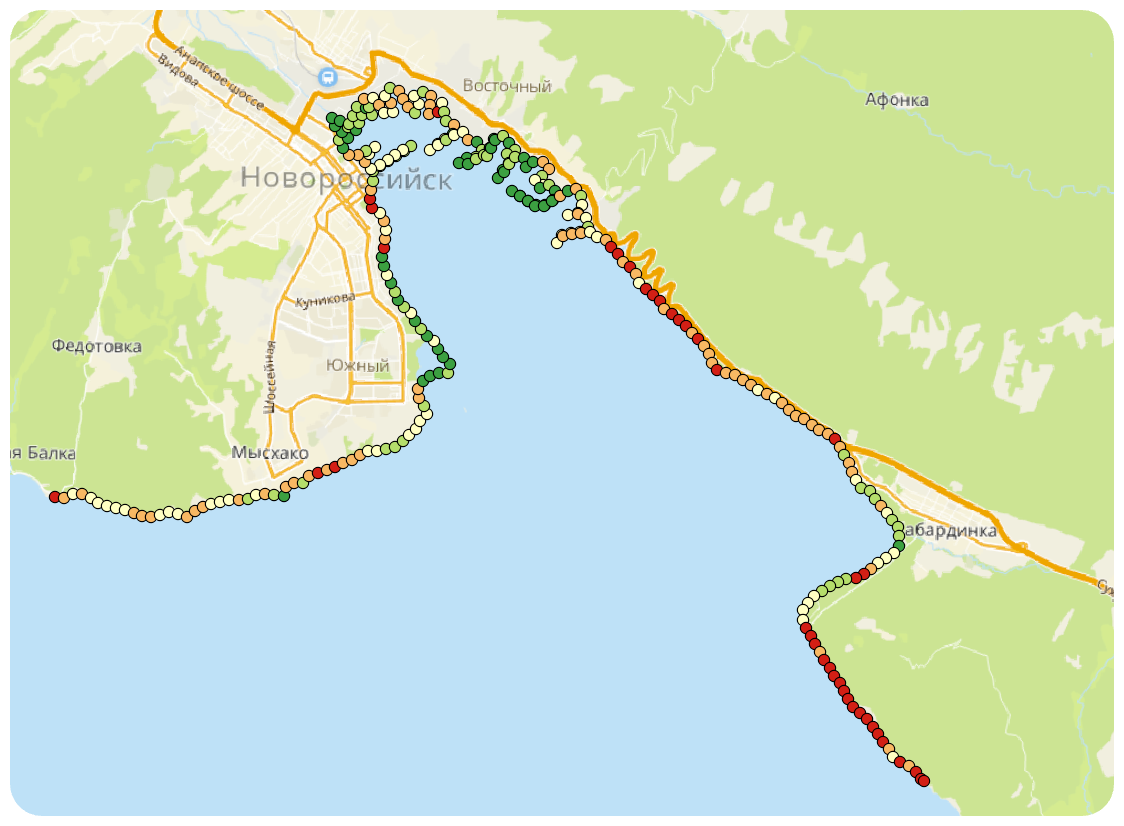
\includegraphics[width=\textwidth]{fig/part_2/NVRSK_WER.png}
	\caption{-- Распределение индекса волновой экспозиции WER в окрестностях г.~Новороссийск}
	\label{pic:NVRSK_WER}
    \end{center}
\end{figure}

В целях упрощения интерпретации этого показателя он был шкалирован по пяти рангам, описанным в таблице~\ref{tab:cwef_percentiles} на странице~\pageref{tab:cwef_percentiles}.
Цветовая палитра была выбрана интутивно понятной -- красный цвет для 5 ранга (самого опасного), зеленый для первого, то есть ранга с минимальным уровнем риска.

Визульно оценивая полученное распределение, можно отметить, что концентрация наиболее опасных участков берега выходит за пределы населенных пунктов, попавших в зону расчета.
Наиболее устойчивые участки берега распределены вдоль Новороссийской набережной и искусственных гидротехнических конструкций, самой надежной из которых оказалась \enquote{клюшка} базы Черноморского военно-морского флота.

Участки берега в районах поселков Кабардинка и Мысхако тоже можно отнести к относительно безопасным.
Тем не менее, что для Новороссийска, что для названных поселков, выделяются локальные, короткие участки берега, сопряженные с зонами повышенного риска проявления негативных гидромеханических явлений.
Оценивая полученные результаты можно сделать вывод, что эволюционным и эмпирическим путем предки выбрали наиболее удачные места для своего расселения.

Тем не менее, несмотря на непротиворечивость введенного индекса реальности и здравому смыслу, он обобщает в себе принципиально разные метрики уязвимости для береговой полосы:
\begin{itemize}
    \item $R_1$ -- средний уровень энергии, характеризующий фоновый уровень волновой нагрузки;
    \item $R_2$ -- штормовую составляющую, характеризующую экстремальную составляющую волновой экспозиции;
    \item $R_3$ -- направленную концентрацию волновой экспозиции, отображающую степень моноориентированности волнового потока;
    \item $R_4$ -- межгодовую изменчивость волновой нагрузки.
\end{itemize}

Рассмотреть распределение этих индексов можно на рисунке~\ref{pic:NVRSK_R1234}.

\begin{figure}
    \begin{center}
	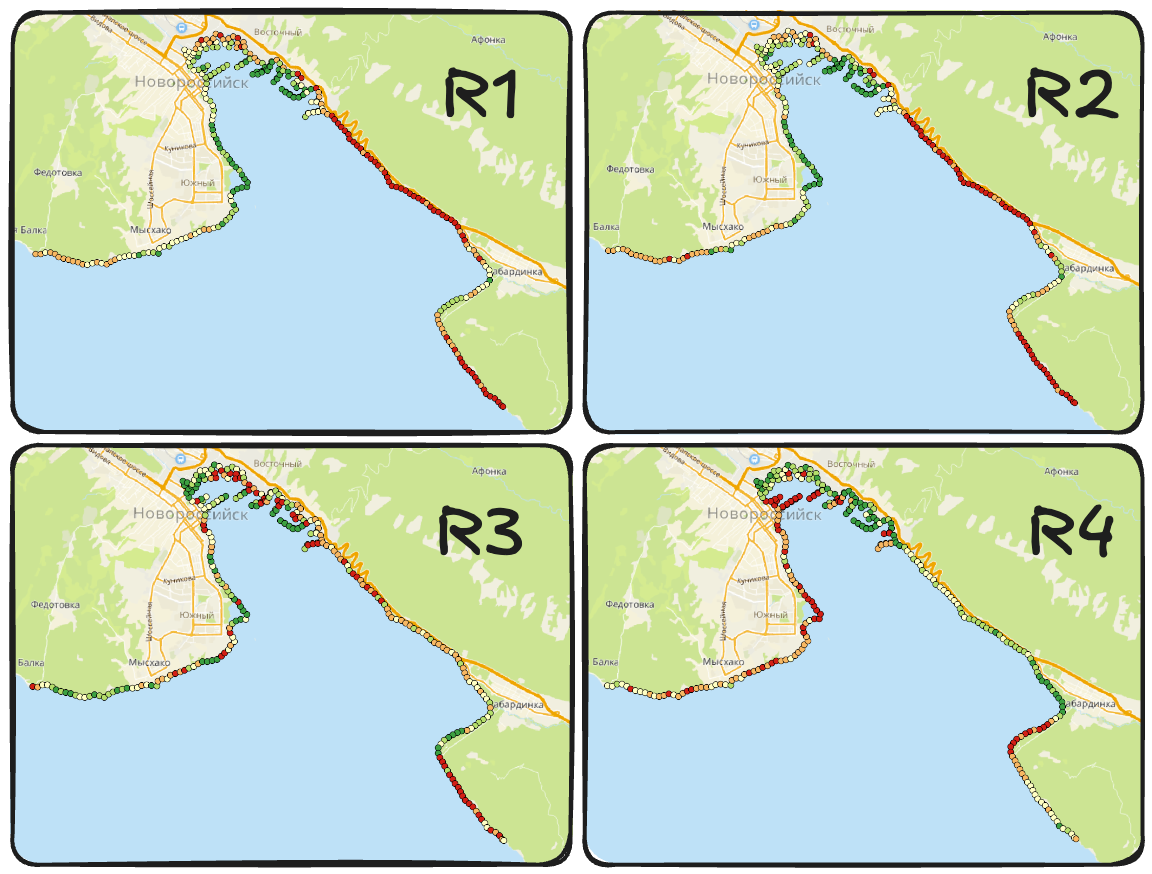
\includegraphics[width=\textwidth]{fig/part_2/NVRSK_R1234.png}
	\caption{-- Распределение рангов волновой уязвимости в окрестностях г.~Новороссийск}
	\label{pic:NVRSK_R1234}
    \end{center}
\end{figure}

Из этого рисунка видно, что распределение индексов $R_1$ и $R_2$ практически эквивалентно.
Это легко объяснить тем, что обрушивающиеся на берег шторма распределены на территории, многократно превышающей зону выполненного анализа.
Распределение наиболе опасных по этим рангам участков беерга находится в пределах автомобильной дороги между Новороссийском и Кабардинкой и \enquote{диким} берегом от Кабардинки в сторону Геленджика.
Можно заметить, что именно эти участки берега наиболее \enquote{открыты} морю, оставаясь незащищенными от воздействия волн.
С другой стороны, открытый морю берег западнее поселка Мысхако обладает меньшими показателями риска в силу отличающейся, практически перпендикулярной, направленности берега, что позволяет сделать вывод о чувствительности выполненных расчетов к изменением топографии местности.

Распределение индекса $R_3$ более вариативно и чуствително к локальной ориентации берега относительно доминирующих направлений ветров.
Наибольшую ценность этот индекс мог бы показать при оценке интенсивности вдольдереговой абразии пляжей, сложенных песчаным материалом.
Скальные породы, из которых сложен берег в рассматриваемом районе, не должны быть сильно уязвимы к этому показателю, отчего интерпретировать его в контексте рассматриваемого случая нет необходимости.

Коэффициент вариации индекса CWEF~\eqref{eq:CWEF} (индекс $R_4$) позволяет увидеть участки берега, на которых распределение волновых нагрузок происходит равномерно во времени.
Так наиболее уязвимые по индексам $R_1$ и $R_2$ участки берега по индексу $R_4$ наиболее устойчивы.
Фактически это можно интрепретировать так, что все, что происходит на этих участках берега, не выходит за пределы нормы для них.
Все худшее, что могло с ними случиться, скорее всего, уже и так случилось и сюрпризом это не станет.
Эти берега находятся в своем естественном равновесии.
При этом городские участки берега подвержены большему риску -- в основное время они закрыты от морских волн и спокойны, но в случае сильного шторма его воздействие выйдет далеко за пределы обычной для них \enquote{нормы}.

Подводя итог, можно сделать вывод, что предлагаемые показатели справляются со своей задачей -- оценить волновое воздействие на берег.
Тем не менее, впереди предстоит большая работа -- необходимо понять, как верно шкалировать и интерпретировать полученные значения, перейдя от эвристических оценок к строгим определениям.

Легко делать выводы по месту где все хорошо (Новороссийск вообще прекрасен), но попробуем применить предложенную методику для города с очевидными проблемами с берегами и набережными -- Выборга.



\subsection{Результаты анализа для Выборга}

\subsubsection{Хронология разрушения набережной в Выборге}

В течение многих лет причальные стенки и ограждения в акватории залива Салакка-Лахти в Выборге эксплуатировались без полноценного капитального ремонта, при этом муниципальные власти фиксировали аварийное состояние отдельных участков набережной. 
Постепенно стало ясно, что проблема носит системный характер и значительная часть набережной находится в неудовлетворительном состоянии.
Доступ к наиболее опасным фрагментам начали ограничивать временными ограждениями (рисунок~\ref{pic:Vyborg_with_crush} \enquote{Г}).

В 2023 году провели инструментальное обследование подводной и надводной частей набережной, по результатам которых подводные конструкции признали аварийными.

К началу лета 2024 года накопленные дефекты конструкций привели к первым крупным обрушениям. 
В начале июня в центре Выборга обвалился участок набережной 30-го Гвардейского корпуса, что привлекло внимание и жителей, и региональных СМИ (рисунок~\ref{pic:Vyborg_with_crush} \enquote{Б}).

После первого обрушения власти детализировали оценку затрат: только затраты на подготовку проектной документации были оценены в десятки миллионов рублей, а полное восстановление всей набережной -- уже в несколько миллиардов.
Фактически это означало, что аварийные участки еще долго будут находиться в режиме временной консервации.

Кульминацией стала вторая волна разрушений летом 2024 года. 
В августе произошло новое обрушение участка набережной в центре города, в районе гостиницы \enquote{Дружба} (рисунок~\ref{pic:Vyborg_with_crush} \enquote{В2}). 
Власти указывали, что доступ к этому участку был закрыт и до инцидента, однако сам факт повторного обрушения подчеркивал критическое состояние всей береговой линии. 

В дополнение отметим, что анализ снимков и публикаций gоказал наличие еще двух локаций с разрушениями набережных, датирующихся более ранним сроком (рисунок~\ref{pic:Vyborg_with_crush} \enquote{А} и \enquote{В1}).

\subsubsection{Результаты расчетов для набережной в Выборге}

Хотя акватория залива Салакка-Лахти не является типичным представителем \enquote{морских} прибрежных территорий математических ограничений для применения предлагаемой методики нет.

На рисунке~\ref{pic:Vyborg_with_crush} показано распределение ранга $R_1$ вдоль городской набережной.

\begin{figure}
    \begin{center}
	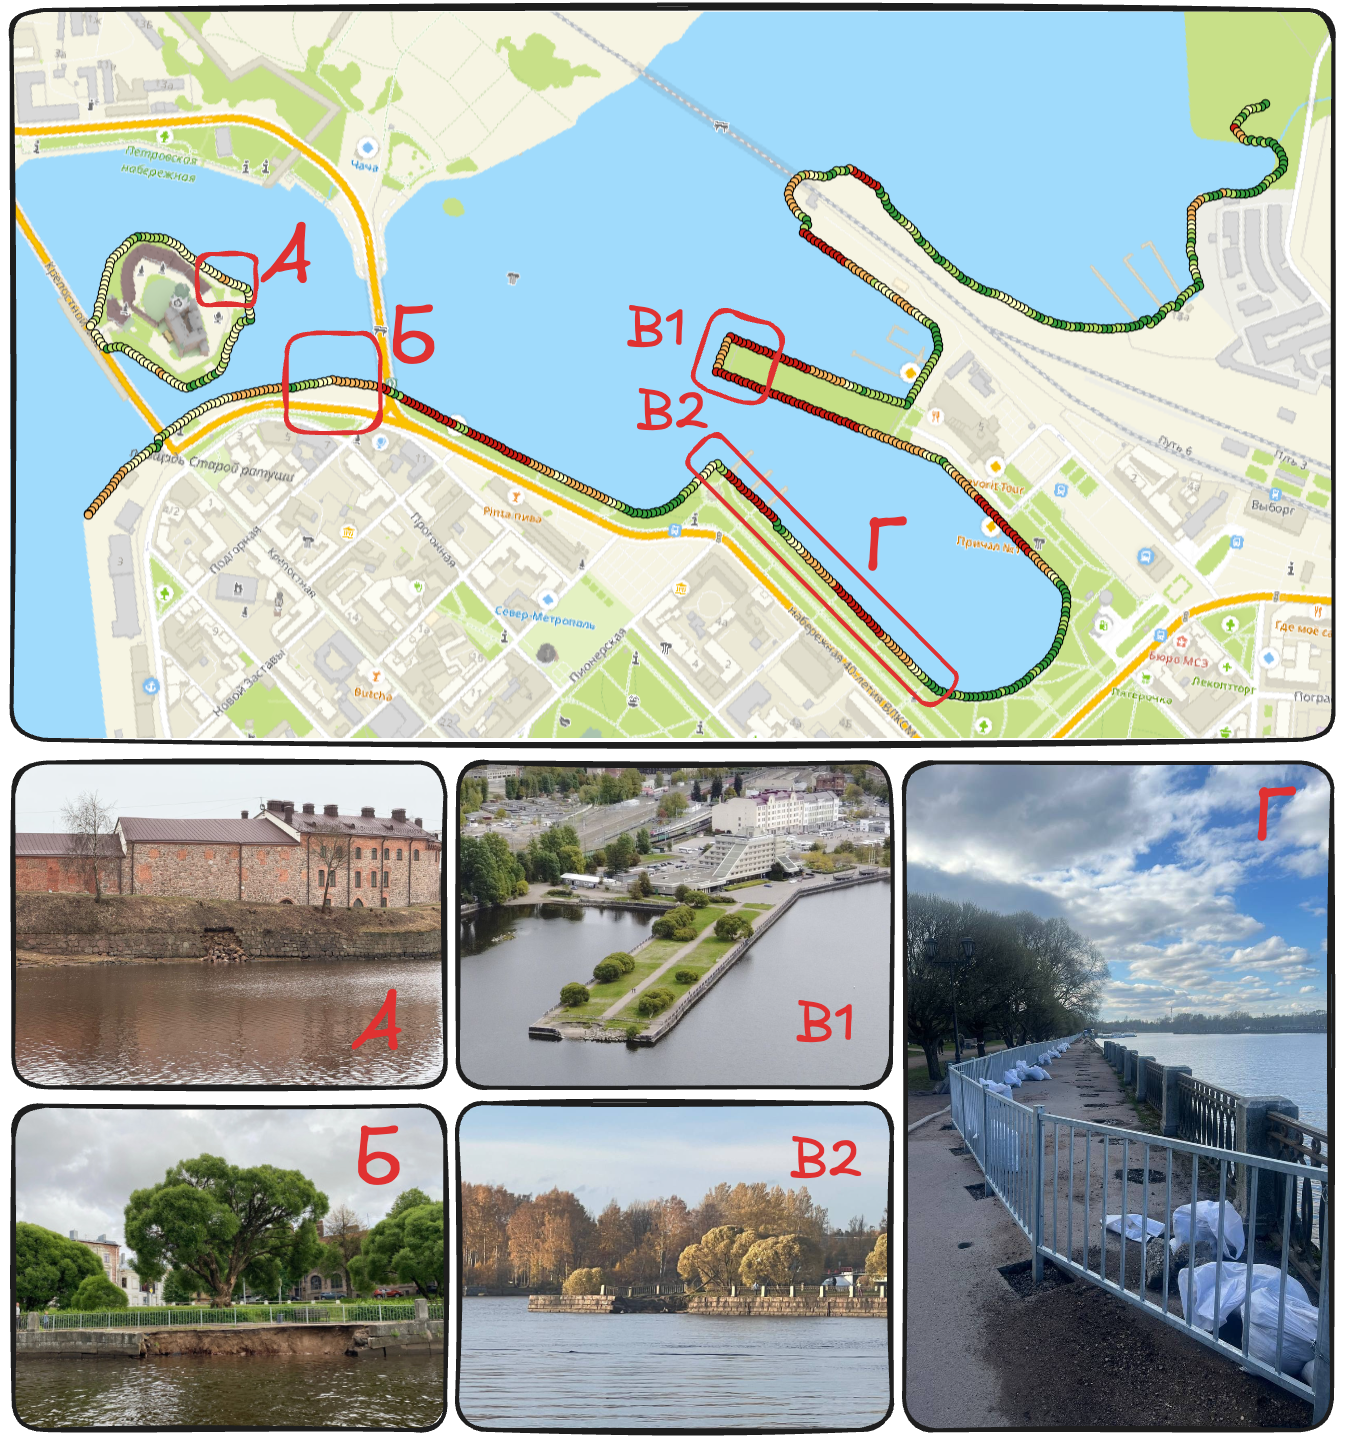
\includegraphics[width=\textwidth]{fig/part_2/Vyborg_with_crush.png}
	\caption{-- Распределение средней волновой нагрузки на набережные г.~Выборг}
	\label{pic:Vyborg_with_crush}
    \end{center}
\end{figure}

Взиуальный анализ распределеиня показывает наличие корреляции высоких показателей индекса с местами проявления аварийных событий.
Отдельно следует отметить, что места аварий определены часто не только высоким показатем индекса (участки \enquote{В} и \enquote{Г}), но и участками с резким измеенением градиента по показателю (участки \enquote{А} и \enquote{Б}).
